% Options for packages loaded elsewhere
\PassOptionsToPackage{unicode}{hyperref}
\PassOptionsToPackage{hyphens}{url}
%
\documentclass[
]{article}
\usepackage{amsmath,amssymb}
\usepackage{lmodern}
\usepackage{ifxetex,ifluatex}
\ifnum 0\ifxetex 1\fi\ifluatex 1\fi=0 % if pdftex
  \usepackage[T1]{fontenc}
  \usepackage[utf8]{inputenc}
  \usepackage{textcomp} % provide euro and other symbols
\else % if luatex or xetex
  \usepackage{unicode-math}
  \defaultfontfeatures{Scale=MatchLowercase}
  \defaultfontfeatures[\rmfamily]{Ligatures=TeX,Scale=1}
\fi
% Use upquote if available, for straight quotes in verbatim environments
\IfFileExists{upquote.sty}{\usepackage{upquote}}{}
\IfFileExists{microtype.sty}{% use microtype if available
  \usepackage[]{microtype}
  \UseMicrotypeSet[protrusion]{basicmath} % disable protrusion for tt fonts
}{}
\makeatletter
\@ifundefined{KOMAClassName}{% if non-KOMA class
  \IfFileExists{parskip.sty}{%
    \usepackage{parskip}
  }{% else
    \setlength{\parindent}{0pt}
    \setlength{\parskip}{6pt plus 2pt minus 1pt}}
}{% if KOMA class
  \KOMAoptions{parskip=half}}
\makeatother
\usepackage{xcolor}
\IfFileExists{xurl.sty}{\usepackage{xurl}}{} % add URL line breaks if available
\IfFileExists{bookmark.sty}{\usepackage{bookmark}}{\usepackage{hyperref}}
\hypersetup{
  pdftitle={PMS Study},
  pdfauthor={Mitchel Kappen \& Sofie Raeymakers},
  hidelinks,
  pdfcreator={LaTeX via pandoc}}
\urlstyle{same} % disable monospaced font for URLs
\usepackage[margin=1in]{geometry}
\usepackage{graphicx}
\makeatletter
\def\maxwidth{\ifdim\Gin@nat@width>\linewidth\linewidth\else\Gin@nat@width\fi}
\def\maxheight{\ifdim\Gin@nat@height>\textheight\textheight\else\Gin@nat@height\fi}
\makeatother
% Scale images if necessary, so that they will not overflow the page
% margins by default, and it is still possible to overwrite the defaults
% using explicit options in \includegraphics[width, height, ...]{}
\setkeys{Gin}{width=\maxwidth,height=\maxheight,keepaspectratio}
% Set default figure placement to htbp
\makeatletter
\def\fps@figure{htbp}
\makeatother
\setlength{\emergencystretch}{3em} % prevent overfull lines
\providecommand{\tightlist}{%
  \setlength{\itemsep}{0pt}\setlength{\parskip}{0pt}}
\setcounter{secnumdepth}{-\maxdimen} % remove section numbering
\ifluatex
  \usepackage{selnolig}  % disable illegal ligatures
\fi

\title{PMS Study}
\author{Mitchel Kappen \& Sofie Raeymakers}
\date{14. September 2021}

\begin{document}
\maketitle

\hypertarget{pms-study}{%
\subsection{PMS Study}\label{pms-study}}

This is the data processing html for the PMS study

kable (tabel, caption = ``table showing the different AIC'')

d0.1 \textless- lmer(Formula,data=data) d0.2 \textless-
glmer(Formula,data=data, family = gaussian(link =
``inverse''),glmerControl(optimizer= ``bobyqa'', optCtrl = list(maxfun =
100000)),nAGQ=0) d0.3 \textless- glmer(Formula,data=data, family =
gaussian(link = ``log''),glmerControl(optimizer= ``bobyqa'', optCtrl =
list(maxfun = 100000)),nAGQ=0)

d0.4 \textless- glmer(Formula,data=data, family = Gamma(link =
``identity''),glmerControl(optimizer= ``bobyqa'', optCtrl = list(maxfun
= 100000)),nAGQ=0) d0.5 \textless- glmer(Formula,data=data, family =
Gamma(link = ``inverse''),glmerControl(optimizer= ``bobyqa'', optCtrl =
list(maxfun = 100000)),nAGQ=0) d0.6 \textless- glmer(Formula,data=data,
family = Gamma(link = ``log''),glmerControl(optimizer= ``bobyqa'',
optCtrl = list(maxfun = 100000)),nAGQ=0)

d0.7 \textless- glmer(Formula,data=data, family = inverse.gaussian(link
= ``identity''),glmerControl(optimizer= ``bobyqa'', optCtrl =
list(maxfun = 100000)),nAGQ=0) d0.8 \textless- glmer(Formula,data=data,
family = inverse.gaussian(link = ``inverse''),glmerControl(optimizer=
``bobyqa'', optCtrl = list(maxfun = 100000)),nAGQ=0) d0.9 \textless-
glmer(Formula,data=data, family = inverse.gaussian(link =
``log''),glmerControl(optimizer= ``bobyqa'', optCtrl = list(maxfun =
100000)),nAGQ=0)

After evaluating different linear models, we found that the best fitting
model for the data is a simple linear model.

Model: PSS \textasciitilde{} PMSScoreNew*TestMoment +
(1\textbar Subject)

\begin{verbatim}
## Analysis of Deviance Table (Type II Wald chisquare tests)
## 
## Response: PSS
##                          Chisq Df Pr(>Chisq)    
## PMSScoreNew             17.199  1  3.367e-05 ***
## TestMoment             245.477  1  < 2.2e-16 ***
## PMSScoreNew:TestMoment 130.346  1  < 2.2e-16 ***
## ---
## Signif. codes:  0 '***' 0.001 '**' 0.01 '*' 0.05 '.' 0.1 ' ' 1
\end{verbatim}

\begin{verbatim}
## Note: D.f. calculations have been disabled because the number of observations exceeds 3000.
## To enable adjustments, add the argument 'pbkrtest.limit = 15752' (or larger)
## [or, globally, 'set emm_options(pbkrtest.limit = 15752)' or larger];
## but be warned that this may result in large computation time and memory use.
\end{verbatim}

\begin{verbatim}
## Note: D.f. calculations have been disabled because the number of observations exceeds 3000.
## To enable adjustments, add the argument 'lmerTest.limit = 15752' (or larger)
## [or, globally, 'set emm_options(lmerTest.limit = 15752)' or larger];
## but be warned that this may result in large computation time and memory use.
\end{verbatim}

\begin{verbatim}
## NOTE: Results may be misleading due to involvement in interactions
\end{verbatim}

\begin{verbatim}
## $emmeans
##  TestMoment emmean    SE  df asymp.LCL asymp.UCL
##           1   30.2 0.142 Inf      30.0      30.5
##           2   29.8 0.143 Inf      29.5      30.1
## 
## Results are averaged over the levels of: PMSScoreNew 
## Degrees-of-freedom method: asymptotic 
## Confidence level used: 0.95 
## 
## $contrasts
##  contrast estimate     SE  df z.ratio p.value
##  1 - 2       0.429 0.0326 Inf  13.146  <.0001
## 
## Results are averaged over the levels of: PMSScoreNew 
## Degrees-of-freedom method: asymptotic
\end{verbatim}

\hypertarget{plots}{%
\subsection{Plots}\label{plots}}

Here are some plots:

\begin{verbatim}
## Warning: Removed 44 rows containing non-finite values (stat_count).
\end{verbatim}

\includegraphics{allPMSdata_files/figure-latex/Plots-1.pdf}
\includegraphics{allPMSdata_files/figure-latex/Plots-2.pdf}
\includegraphics{allPMSdata_files/figure-latex/Plots-3.pdf} with
PMSScore=0 and testmoment = 2 there seem to be some outliers This means
that people with low PMS scores had more outliers on testmoment 2. we
might need to remove some of these outliers

Some extra pilot plots

\begin{verbatim}
## [1] "we have more participants with low PMS score"
\end{verbatim}

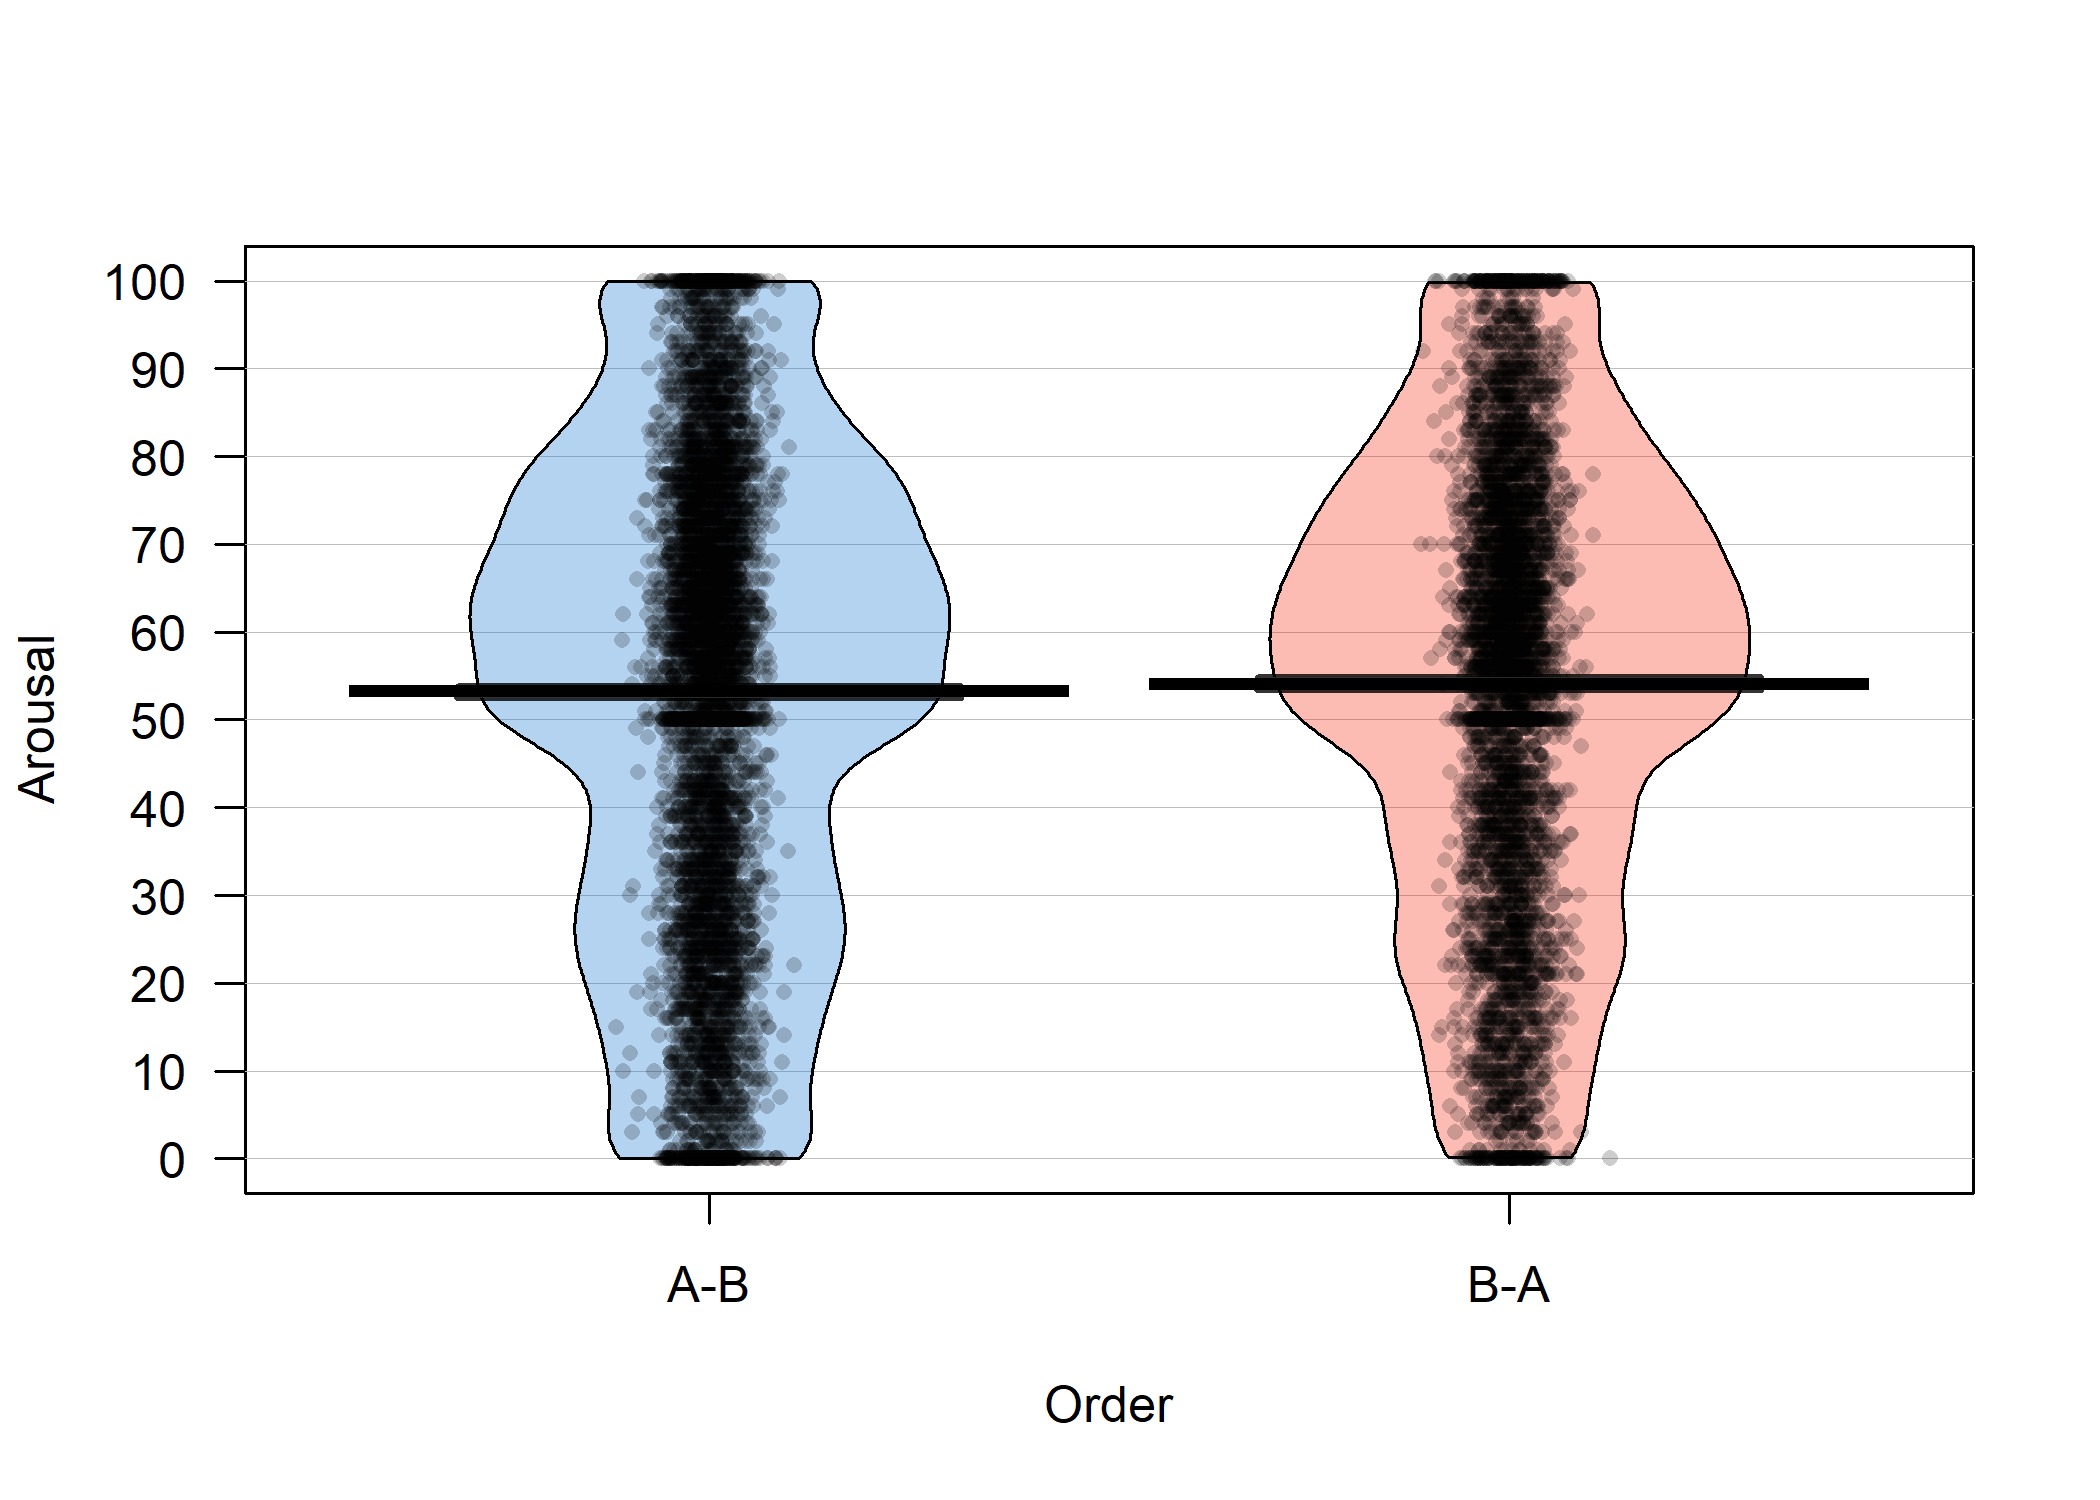
\includegraphics{allPMSdata_files/figure-latex/unnamed-chunk-1-1.pdf}
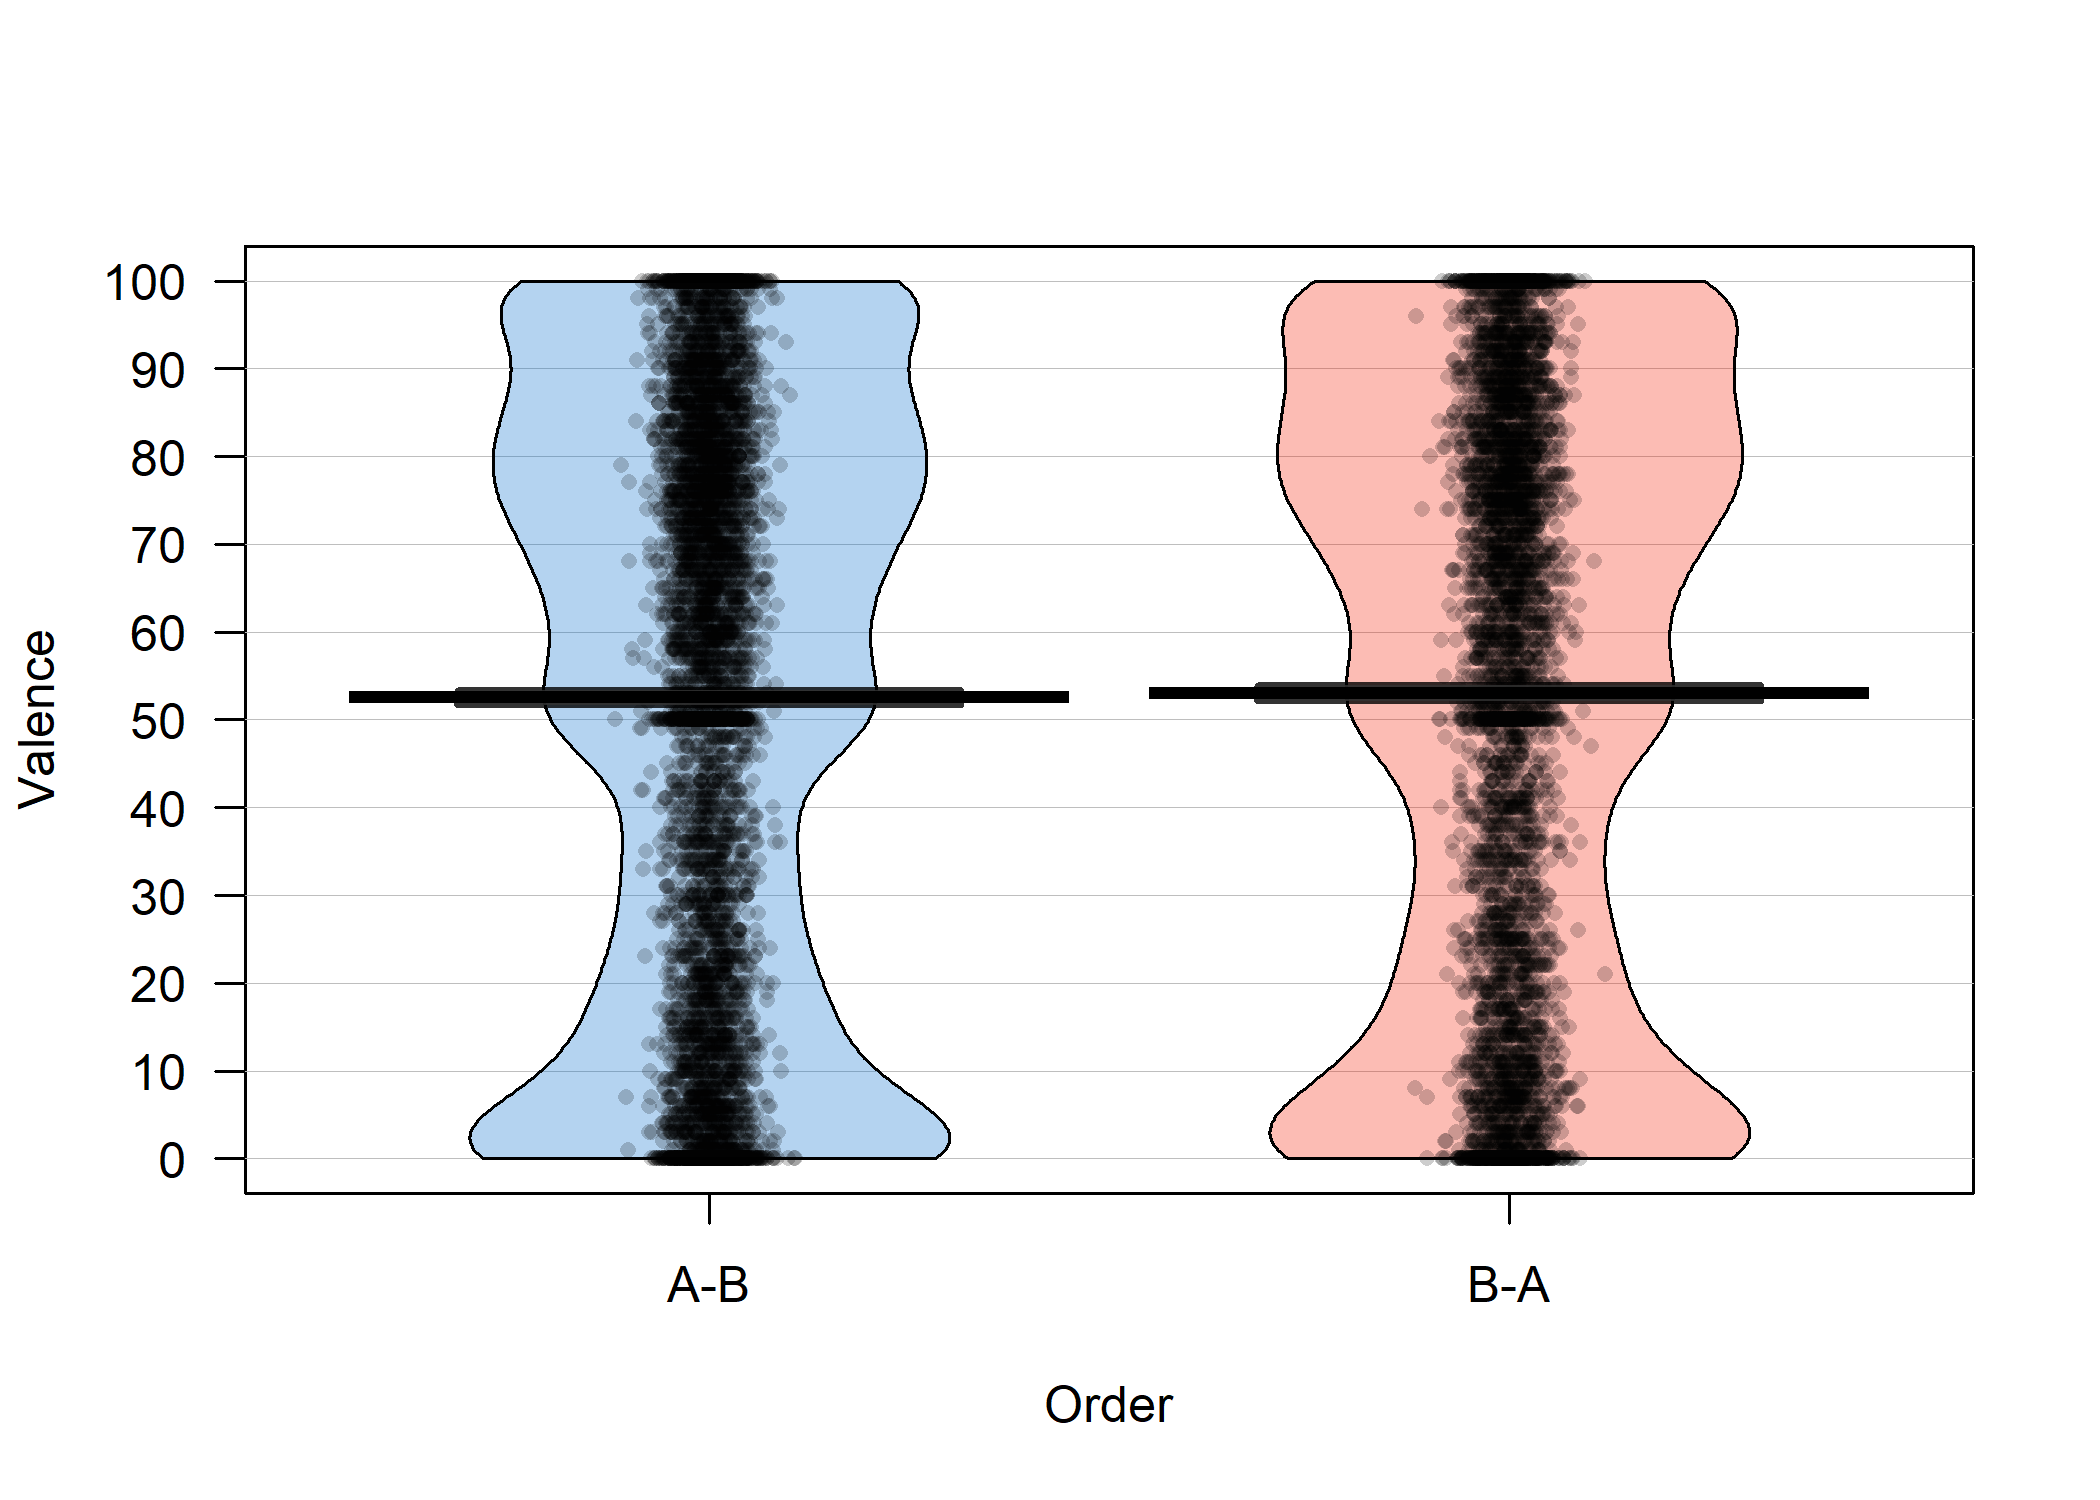
\includegraphics{allPMSdata_files/figure-latex/unnamed-chunk-1-2.pdf}

\begin{verbatim}
##    Min. 1st Qu.  Median    Mean 3rd Qu.    Max.    NA's 
##   10.00   28.00   30.00   29.85   32.00   40.00      44
\end{verbatim}

There are 9328 people with low PMS score and 6468 people with high PMS
score

The mean age is 31.7

The End!

\end{document}
